\newpage
\section{Part 2: Testing hardware, configuration and logic}
\subsection{Hardware test by downloading}
\begin{itemize}
    \item{Configuration downloaded}
    \item{OPC Server updated}
    \item{Tags exported}
    \item{Valve tested in Online-mode (0-100\%)}
\end{itemize}


The valve functions as intended, but the pressure transmitter (PT) needs some calibration according to the level glas (LG).

\textbf{Old parameters:}

$EU\_100 = 690$

$EU_\_0 = 240$

\textbf{New parameters:}

$EU\_100 = 435$

$EU_\_0 = 170$






\subsection{Logic Configuration}
We created an Analog Out (AO) block in the CurrentConverter controlling the valvle, and an Analog Input (AI) block in the PressureTransmitter giving input to the PID on present value (PV).

According to the assignment text, we should have chosen one of the nodes to include the PID controller. After a little bit of experimenting, we reasoned with that it could be implemented in both modules, and also directly into the application if the module attachments were done properly.

The PID parameters was setup as described in the assignment text.

When it comes to the control strategy, we connected the blocks accordingly to:
\begin{itemize}
    \item{AI.OUT to PID.IN}
    \item{PID.OUT to AO.CAS-IN}
    \item{AO.BKCAL\_OUT til PID.BKCAL\_IN}
\end{itemize}

\subsection{Logical testing and regulator tuning}
This section resulted in a lot of testing and troubleshooting.

The Pressure Transmitter provided an output signal of 0 to -100 compared to the level glas, which made us want to invert that output. After some reading of documentation we found the invert-function, though it did not work as documented. We also experimented with arithmetic blocks to multiply the signal with a factor $K = -1$, but the result was unsuccesfull. 
Could this problem be caused by inverted polarity?

The software did neither accept the limits of 0 to -100 \%, which again made this final task very difficult.

If the signal had been positive, it would have been a simple task to tune the regulator with Ziegler-Nichols method, but due to this issue, it did not work as intended.

If the level was approximately 50\%, the transmitter provided an output signal of -50. When the set-value was defined positive from 0-100\%, the PID would just open the valve more and more due to increasing deviation as the level output rised towards -100\%.

After almost 10 hours at the lab, experimenting with different parameters in all modules, we concluded that there must be some modification to be done, to make the signal positive instead of negative.

\begin{figure}[!htb]
    \centering
    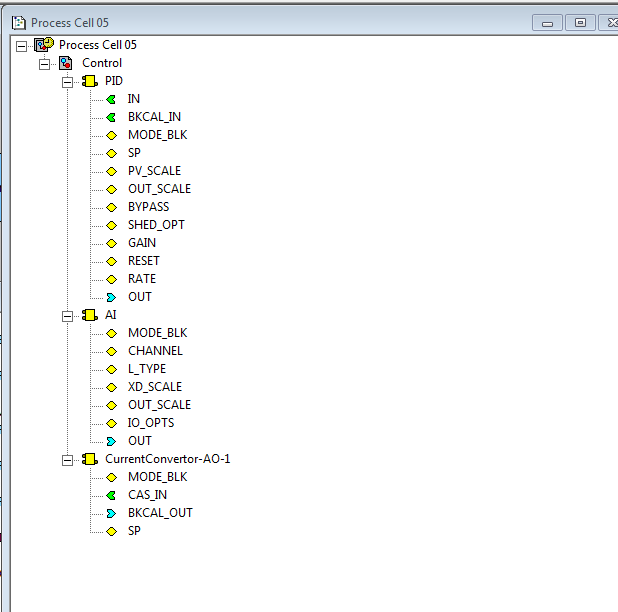
\includegraphics[width=0.7\textwidth]{images/PId_Process}
    \caption{Change of Rev.}
    \end{figure}
    
    
\begin{figure}[!htb]
    \centering
    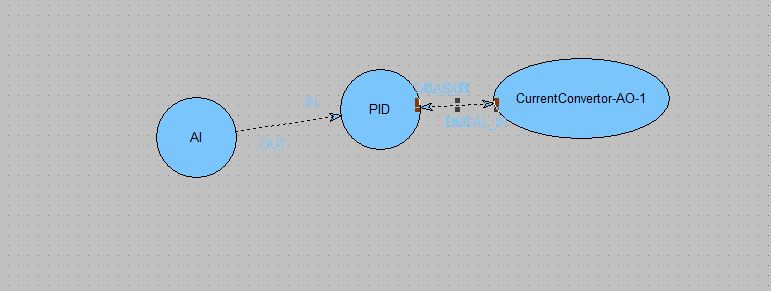
\includegraphics[width=0.7\textwidth]{images/ControlPID}
    \caption{Change of Rev.}
    \end{figure}

